\label{chap:testing}
\section{PolyBench}
The framework is tested with polyBench 1.0 and the results are shown in the next section.
PolyBench, a set of computation intensive programs often used in the polyhedral community.
On those benchmarks Polly extracts the relevant SCoPs and optimizes them automatically.

\section{Experimental results}

The OpenMP code generated by Polly is compared with gcc and graphite\cite{TRIFUNOVIC:2010}. With gcc
we make a comparison with serial execution and with graphite we make comparison
with an existing autoparallelization framework, which is also based on polyhedral
model.

The script for testing is given below
{\footnotesize
\begin{verbatim}
# serial
gcc -I utilities utilities/instrument.c -DPOLYBENCH_TIME 
                      -DPOLYBENCH_DUMP_ARRAYS -O3 $1 -lm
# Autopar with graphite
gcc -I utilities utilities/instrument.c -DPOLYBENCH_TIME
           -DPOLYBENCH_DUMP_ARRAYS -O3 -floop-interchange
           -floop-block -floop-parallelize-all 
	   -ftree-parallelize-loops=2 $1 -lm
# Autopar with polly OpenMP
pollycc -fpolly -fparallel -I utilities utilities/instrument.c
              -DPOLYBENCH_TIME -DPOLYBENCH_DUMP_ARRAYS  $1 -lm
\end{verbatim}
}
\begin{figure}
\begin{center}
  \label{fig:2core1}
  %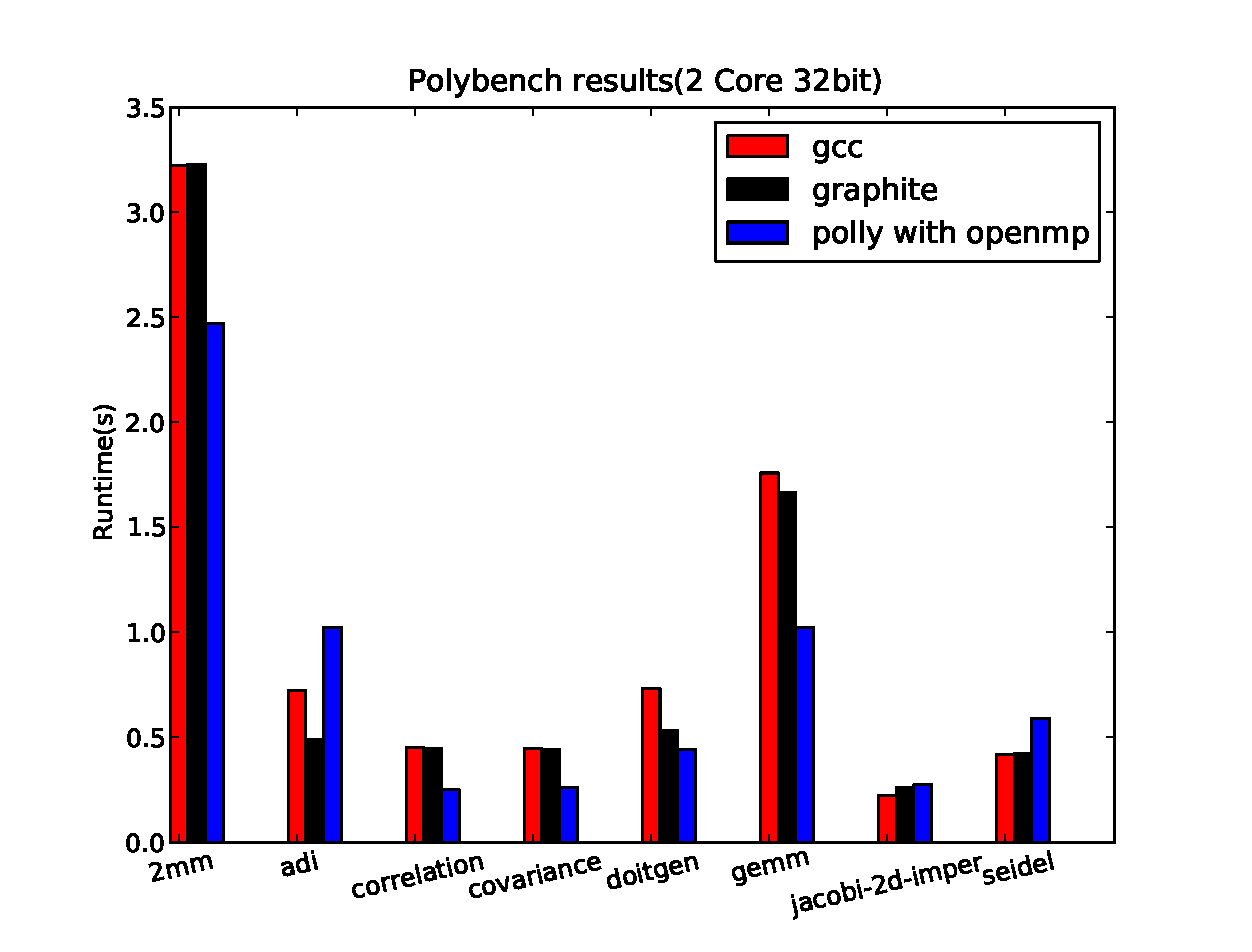
\includegraphics[width=1\textwidth]{images/2core32bit.eps}
  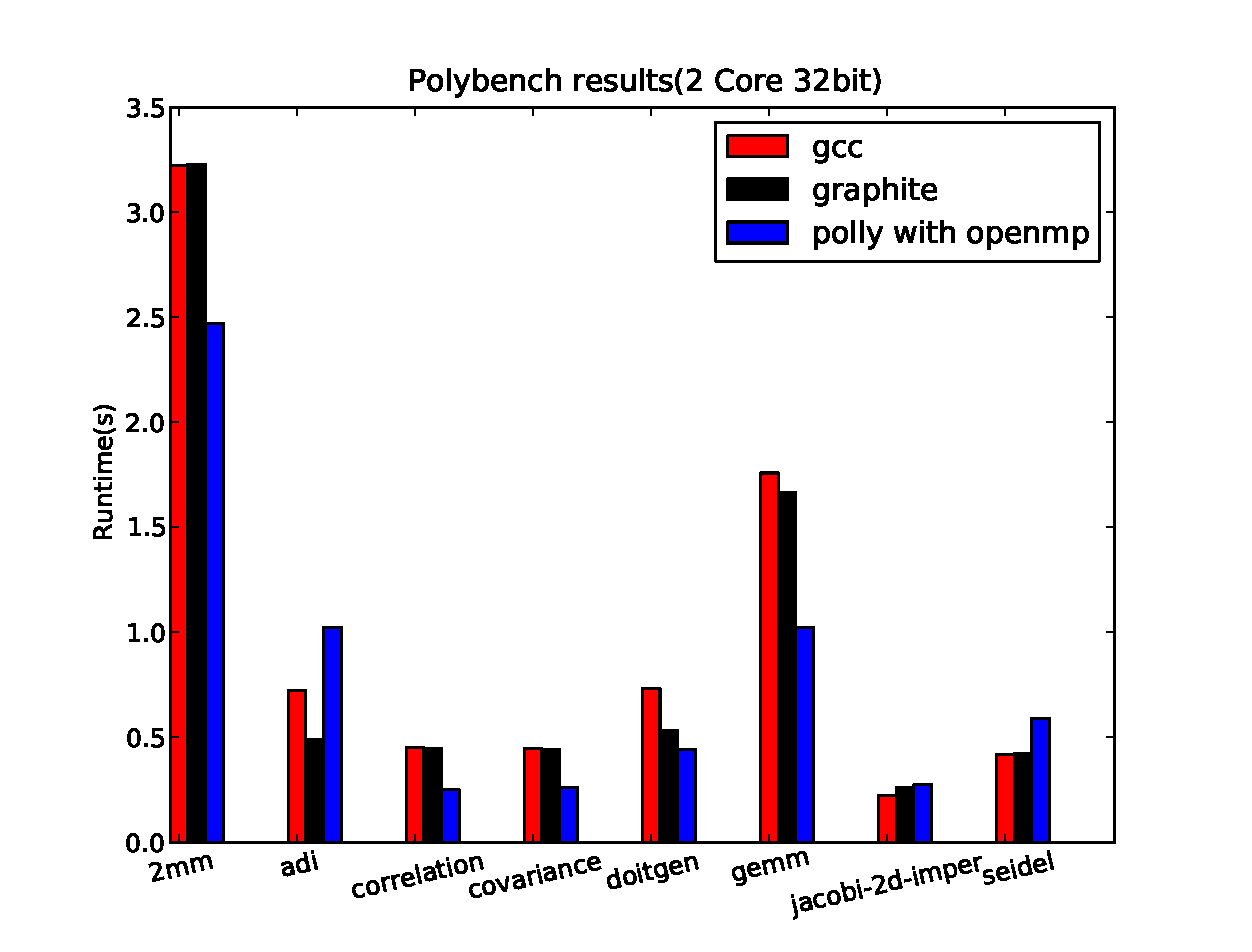
\includegraphics[height=9cm]{images/2core32bit.eps}
  \caption{Performance comparison}
\end{center}
\end{figure}

\begin{figure}
\begin{center}
  \label{fig:2core2}
  %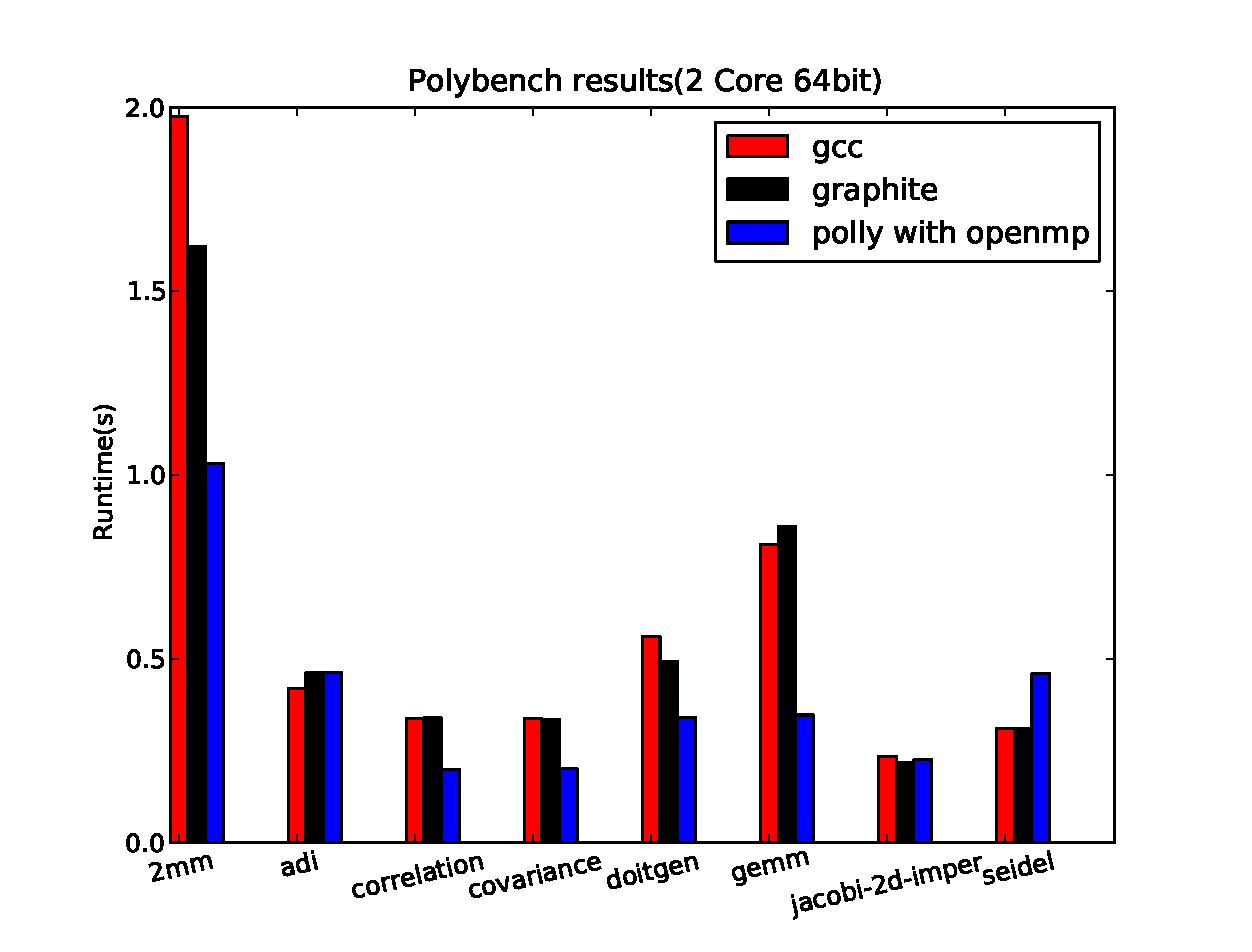
\includegraphics[width=1\textwidth]{images/2core64bit.eps}
  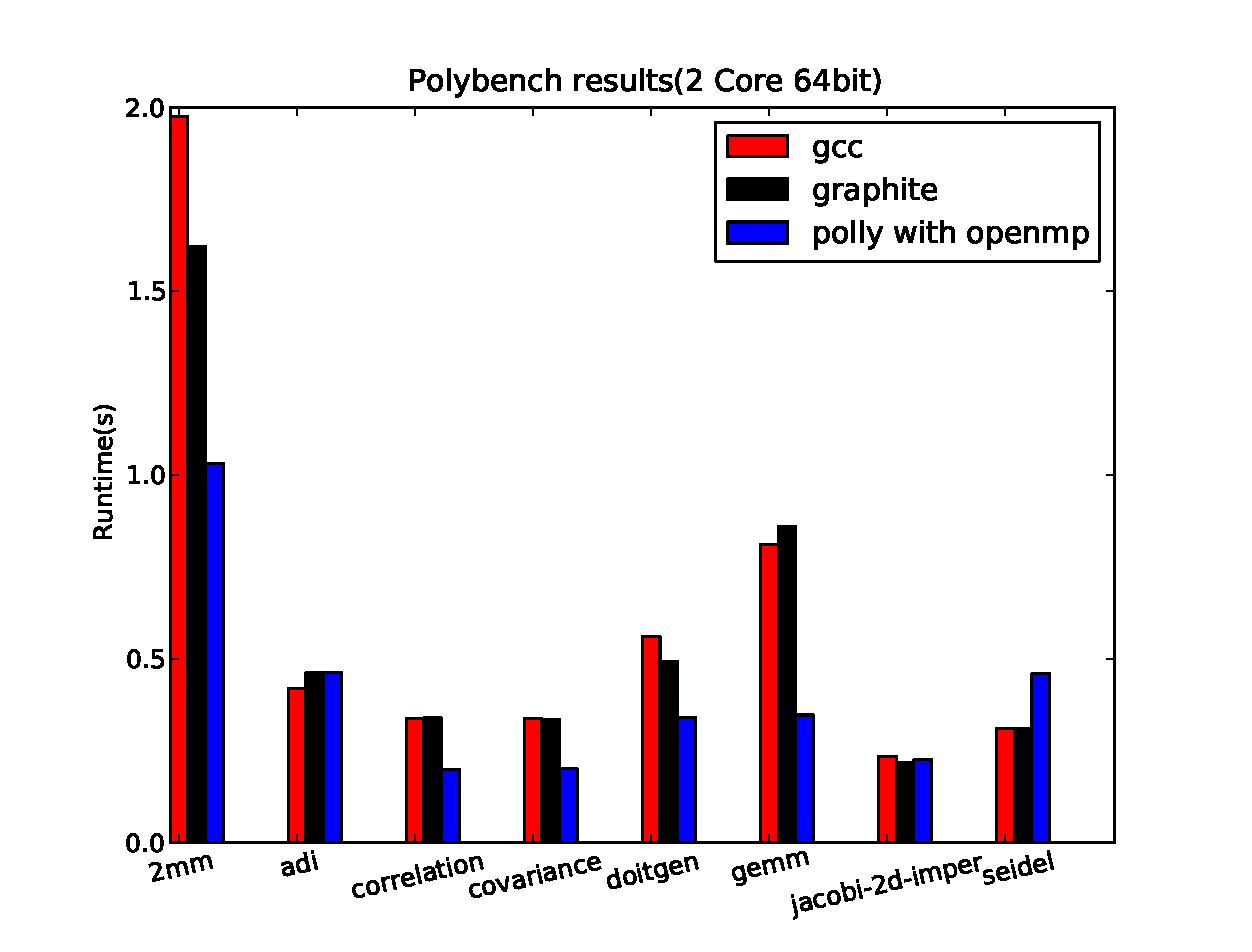
\includegraphics[height=10cm]{images/2core64bit.eps}
  \caption{Performance comparison}
\end{center}
\end{figure}

\begin{figure}
\begin{center}
  \label{fig:10core}
  %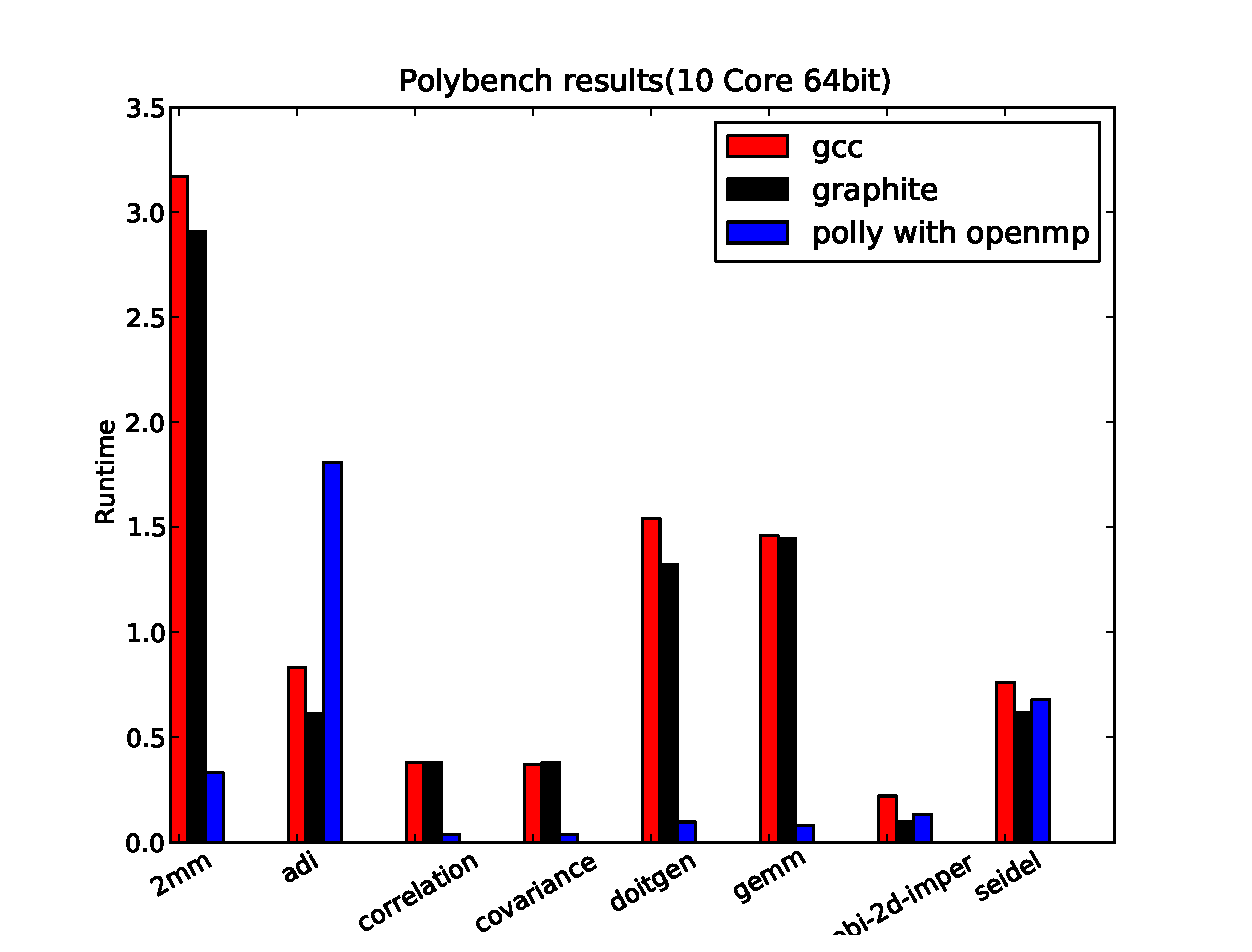
\includegraphics[width=1\textwidth]{images/10core64bit.eps}
  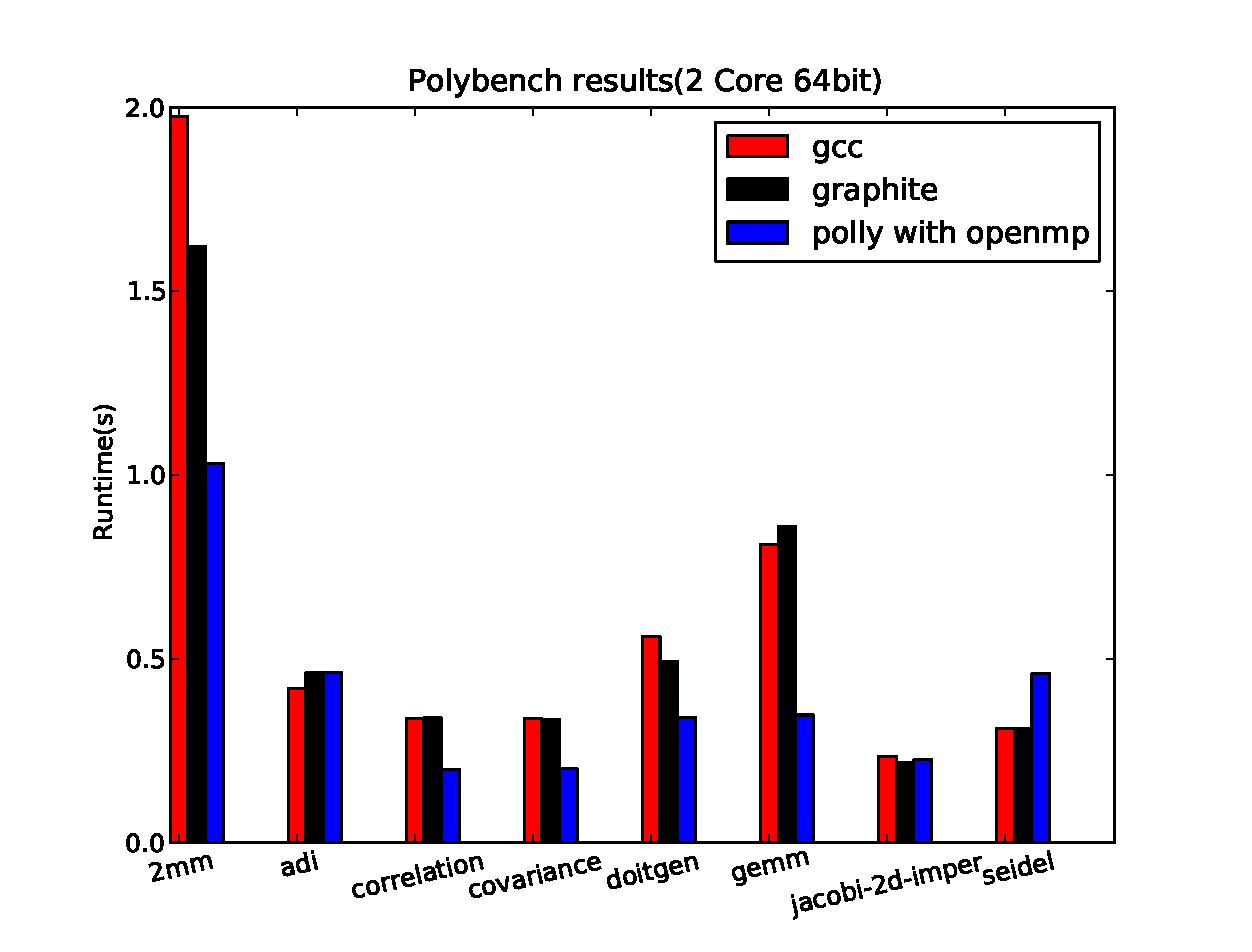
\includegraphics[height=10cm]{images/2core64bit.eps}
  \caption{Performance comparison}
\end{center}
\end{figure}
